\documentclass[cn]{homework}

\title{作业1}

\begin{document}
    \maketitle

    \section{题1}

    我们先将\colorbox{lbcolor}{\lstinline{DATE}}转换为日期类型
    \begin{lstlisting}
        gen double DATE_REAL = quarterly(DATE, "YQ")
    \end{lstlisting}
    然后使用\code{summarize}得到一些描述性统计结果
    \begin{figure}[h]
        \centering
        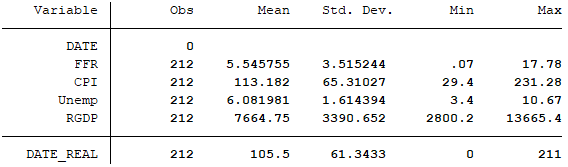
\includegraphics[width=0.7\textwidth]{summarize.png} 
        \caption{基本统计量}
    \end{figure}

    再分别通过以下的命令画出散点图
    \begin{lstlisting}
        graph twoway scatter FFR DATE_REAL
        graph twoway scatter CPI DATE_REAL
        graph twoway scatter Unemp DATE_REAL
        graph twoway scatter RGDP DATE_REAL
    \end{lstlisting}

    \begin{figure}[h]
        \centering
        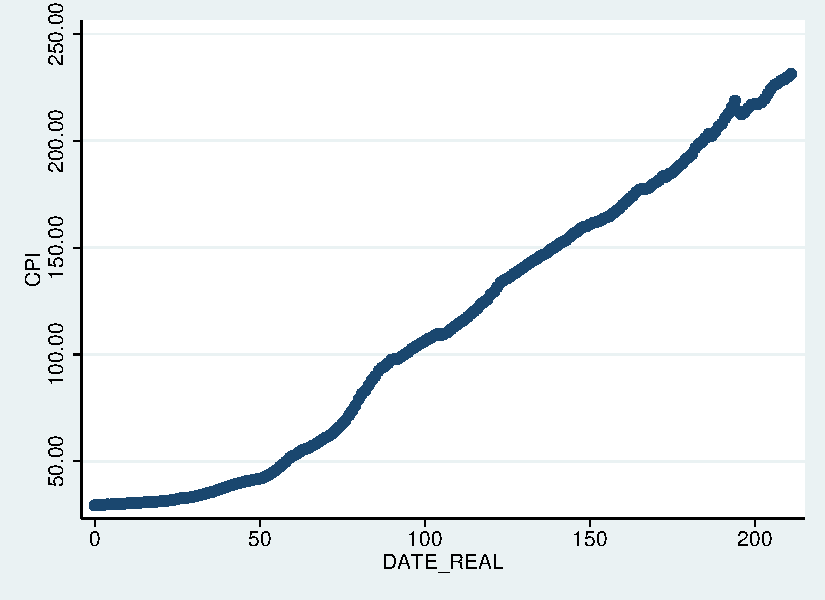
\includegraphics[width=0.4\textwidth]{CPI.pdf}
        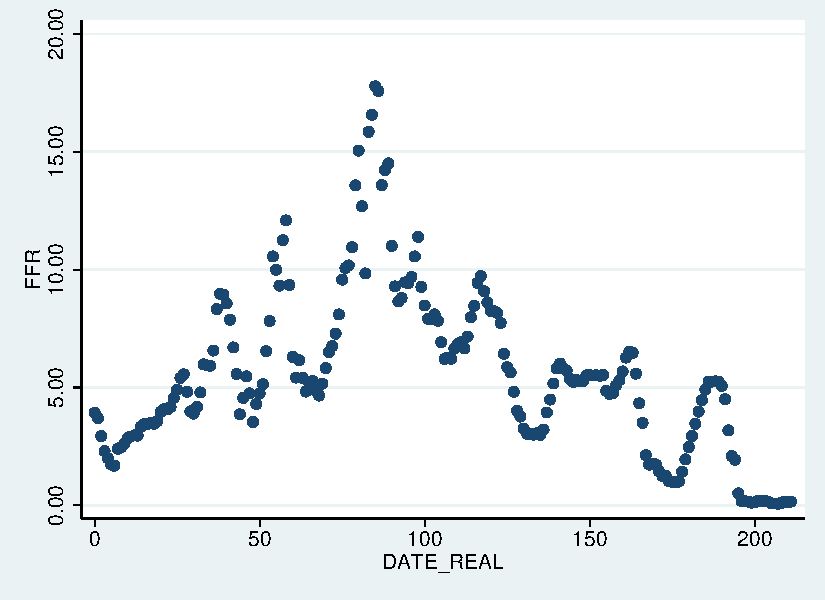
\includegraphics[width=0.4\textwidth]{FFR.pdf}
        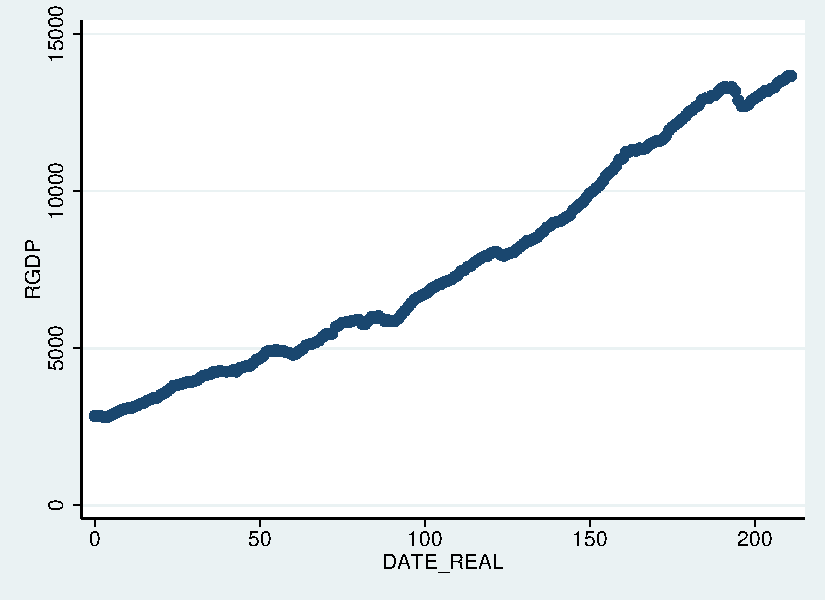
\includegraphics[width=0.4\textwidth]{RGDP.pdf}
        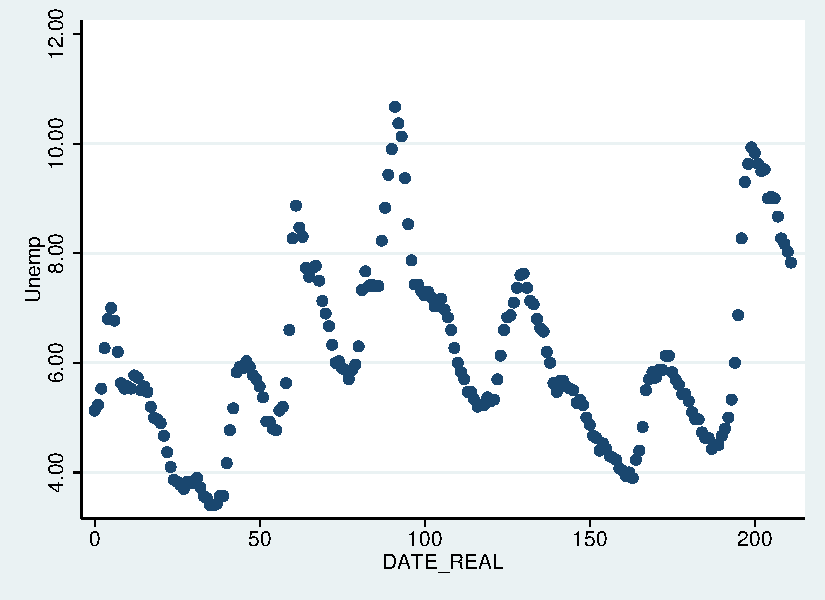
\includegraphics[width=0.4\textwidth]{Unemp.pdf}
        \caption{散点图}
    \end{figure}

    不难发现
    \begin{enumerate}
        \item 
        CPI和RGDP整体呈现上升趋势,且除了CPI在前50个季度内上升
        幅度较小,其他时期两者几乎呈现出线性增长的趋势。

        \item
        Unemp呈现周期性的趋势,一个小周期大约25个季度,同时大约
        有一个60季度长的大周期。

        \item
        FFR的变化稍稍没那么有规律,也能大概看有20季度左右的小周期,
        同时在第90个季度左右达到了一个较长时间内的峰值,随后总体趋势
        下降。

    \end{enumerate}

    \section{题2}
    \begin{proof}
        % 首先考察$X(t)$的期望,
        % 由白噪声序列的定义知期望存在且$E\varepsilon_i=u$为一与下标无关的常量。
        % 而$\sum |a_i|<\infty$即序列绝对收敛,故
        % \begin{align*}
        %     EX(t)&=E(\sum a_i\varepsilon_{t-i})\\
        %          &=\sum a_iE\varepsilon_{t-i}\\
        %          &=u\sum a_i < \infty
        % \end{align*}
        % 亦为与时间无关的常量。


    %     对于任意的$t,s\in\mathbb N$,不妨设$t-s=d\geq 0$,考虑协方差
    %     \begin{align*}
    %         \mathrm{Cov}(X(t),X(s))&=\mathrm{Cov}(\sum a_i\varepsilon_{t-i},\sum a_j\varepsilon_{s-j})\\
    %     \end{align*}

    %     又由$\{\varepsilon_i\}$为白噪声序列,则
    %     \[\mathrm{Cov}(\varepsilon_i,\varepsilon_j)=\begin{cases}
    %         \sigma^2,&i=j\\
    %         0,       &i\neq j
    %     \end{cases}\]
    %     这里$\sigma^2$为一个与$i,j$无关的常数。

    %     又由极限的保号性和幂函数的连续性
    %     \[\sum_{i-j=d}a_ia_j\leq\lim_{n\to\infty}\left(\sum_{i=0}^n|a_i|\right)^2
    %     <\infty\]

    %     因此
    %     \begin{align*}
    %         \mathrm{Cov}(X(t),X(s))&=\mathrm{Cov}(\sum a_i\varepsilon_{t-i},\sum a_j\varepsilon_{s-j})\\
    %                                &=\sum_{t-i=s-j}a_ia_j\mathrm{Cov}(\varepsilon_{t-i},\varepsilon_{s-j})\\
    %                                &=\sigma^2\sum_{i-j=d}a_ia_j
    %     \end{align*}
    %     即协方差仅与$t,s$的差$d$有关,具有平移不变性。

    %     因此$\{X(t)\}$为宽平稳序列。
    \end{proof}
\end{document}